
%\subsection{solución}

%Para llevar a cabo lo expuesto anteriormente %en el planteamiento del problema
Para esto, se plantea la implementación de un sistema capaz de tomar datos de forma continua y enviarlos a un servidor el cual permita el almacenar, estudiar y muestrear la información en distintos niveles de profundidad, con respecto al análisis realizado.\\
Para esto se plantea una simulación digital, diagramada en la figura \ref{fig:diagrama}, que constara de un análisis estadístico para obtener las medidas típicas de un acelerómetro en motores eléctricos con distintos niveles de daños, esta data permitirá, después de ser almacenada en una base de datos y procesada, generar 3 niveles de análisis:\\
\begin{itemize}
\item La vista principal, permitirá observar una cantidad especifica de motores, simbolizando los existentes en una planta o piso, y su estado general.

\item La vista especifica, dará la información actual e histórica referente a un único motor previamente seleccionado.

\item La vista exhaustiva se refiere a un análisis en frecuencia de la vibración de un motor especificado con anterioridad, con la finalidad de permitir al operador o ingeniero encargado determinar la causa de las posibles averías.
\end{itemize}


Y finalmente, toda esta información y opciones se mostrarían a través de una pagina web para facilitar su acceso.

\begin{figure}[htb]
\centering
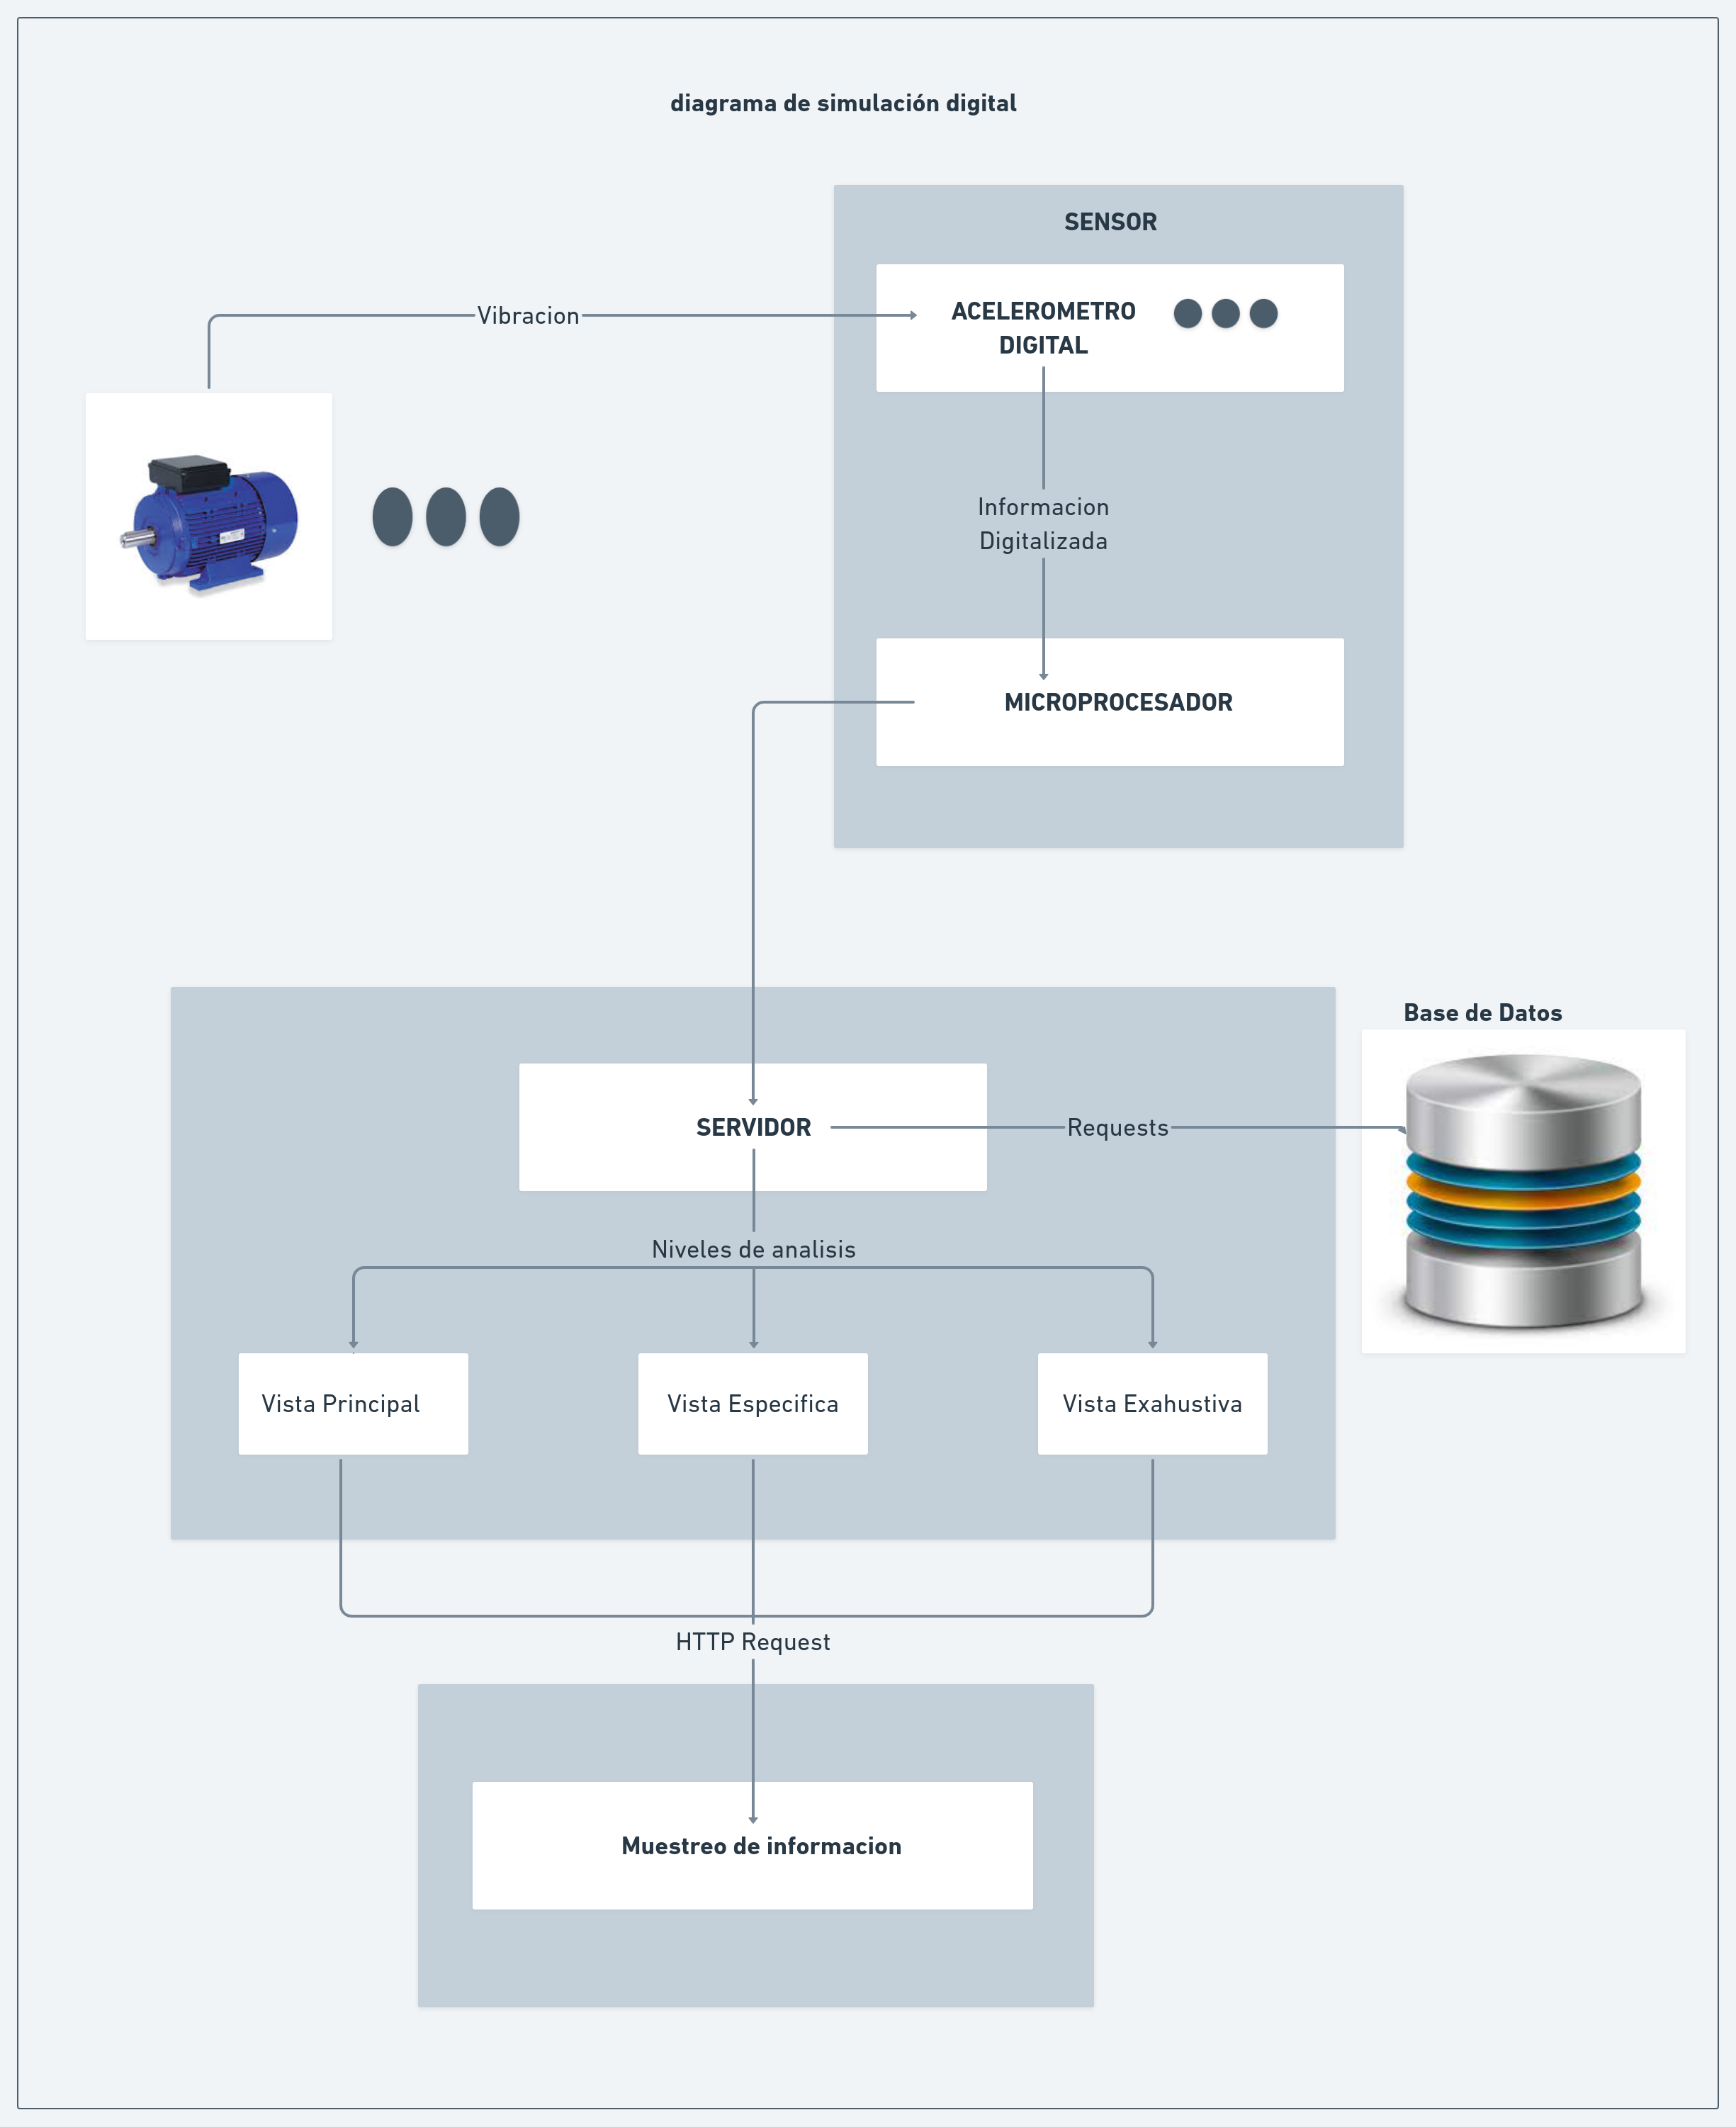
\includegraphics[width=15cm]{Diagrama_sensorica.png}
\caption{Diagrama de la simulación digital}
\label{fig:diagrama}
\end{figure}


